\documentclass[utf8,compress]{beamer}
\usepackage{irbookslide}
\usepackage{irilmenau2}
\usepackage{url}
\usepackage{fontspec} % zahteva paket euenc
\usepackage{xunicode}
\usepackage{xltxtra}
\usepackage{polyglossia}
\usepackage[cache=false]{minted}
\usepackage{xcolor,colortbl}
\usepackage{textcomp}
\usepackage{unicode-math}

\title{Objektno-orijentisano programiranje i Python}
\subtitle{\tiny{Slajdovi za predmet Osnove programiranja}}
\subject{Osnove programiranja}
\institute{Katedra za informatiku, Fakultet tehničkih nauka, Novi Sad}
\date{2018.}

\begin{document}
% da pygmentize ne uokviruje crvenom bojom nepoznate karaktere
\expandafter\def\csname PY@tok@err\endcsname{}

\frame{\titlepage}

\frame{
  \frametitle{Ciljevi}
  \begin{itemize}
    \item savlađivanje osnovnih pojmova objektno-orijentisanog programiranja
  \end{itemize}
}

\section[Klasa i objekat]{Klasa i objekat}

\begin{frame}[fragile]
  \frametitle{Pojam objekta}
  \begin{itemize}
    \item \myblue{objekat} je akter u realnom sistemu koji opisujemo programom
    \item na primer, naš program treba da rukuje dužima i krugovima u Dekartovom koordinatnom sistemu
    \item šta je duž? šta je krug?
    \begin{itemize}
      \item matematička definicija: skup tačaka koje...
      \item programerska definicija: koji podaci su nam dovoljni da opišu duž ili krug?
    \end{itemize}
  \end{itemize}
\end{frame}

\begin{frame}[fragile]
  \frametitle{Pojam objekta $_2$}
  \begin{itemize}
    \item duž je određena pomoću dve krajnje tačke
    \item krug je određen centrom (tačka) i poluprečnikom
    \item tačka je određena Dekartovim koordinatama
    \item $\Rightarrow$ tačka je \myblue{objekat} opisan svojim koordinatama
    \item program može da rukuje sa više tačaka istovremeno
    \item \textbf{svaka tačka} biće poseban objekat
    \item šta je zajedničko svim tačkama?
    \begin{itemize}
      \item struktura (podaci kojima su opisane)
      \item ponašanje (operacije nad njima) 
    \end{itemize}
  \end{itemize}
\end{frame}

\begin{frame}[fragile]
  \frametitle{Pojam klase}
  \begin{itemize}
    \item strukturu i ponašanje svih tačaka opisaćemo na jednom mestu
    \item taj opis nazvaćemo \myblue{klasa}
    \item klasa predstavlja novi tip podataka
    \item konkretni \textbf{objekti} su \myblue{instance} (primerci) \textbf{klase}
  \end{itemize}
\end{frame}

\begin{frame}[fragile]
  \frametitle{Pojam klase $_2$}
\begin{minted}{python}
class Point: # klasa Point opisuje sve tacke u programu
    def __init__(self, x, y):
        self.x = x
        self.y = y
    def equals(self, other):
        return self.x == other.x and self.y == other.y

a = Point(5, 3)  # a je objekat klase Point
b = Point(3, 4)  # b je objekat klase Point
c = Point(5, 3)  # c je objekat klase Point
print(a.equals(b))
print(a.equals(c))
\end{minted}
\end{frame}

\begin{frame}[fragile]
  \frametitle{Pojam klase}
  \begin{itemize}
    \item \myblue{atributi} klase: podaci koji opisuju stanje objekta
    \begin{itemize}
      \item atributi klase \texttt{Point}: \texttt{x}, \texttt{y}
    \end{itemize}
    \item \myblue{metode} klase: funkcije koje opisuju ponasanje objekta
    \begin{itemize}
      \item metode klase \texttt{Point}: \texttt{equals}
    \end{itemize}
  \end{itemize}
\end{frame}

\begin{frame}[fragile]
  \frametitle{Šta je \texttt{self}}
\begin{minted}{python}
class Point:
    def __init__(self, x, y):
        self.x = x
        self.y = y
    def equals(self, other):
        return self.x == other.x and self.y == other.y
\end{minted}
  \begin{itemize}
    \item \texttt{self} označava onaj objekat čija metoda je pozvana
    \begin{itemize}
      \item self = ``ja''
    \end{itemize}
    \item \texttt{self.x}: vrednost mog atributa \texttt{x}
    \item \texttt{other.x}: vrednost atributa \texttt{x} objekta \texttt{other}
  \end{itemize}
\end{frame}

\begin{frame}[fragile]
  \frametitle{Šta je \texttt{self} $_2$}
  \begin{itemize}
    \item ko je \texttt{self} a ko je \texttt{other}?
  \end{itemize}
\begin{minted}{python}
print(a.equals(b))
\end{minted}
  \begin{itemize}
    \item poziva se metoda \texttt{equals} objekta \texttt{a}
    \item parametar poziva metode je objekat \texttt{b}
    \item \texttt{a} je \texttt{self}
    \item \texttt{b} je \texttt{other}
  \end{itemize}
\end{frame}

\begin{frame}[fragile]
  \frametitle{Šta je \texttt{self} $_3$}
  \begin{itemize}
    \item prvi parametar svake funkcije koja je deo klase je \texttt{self}
  \end{itemize}
\begin{minted}{python}
class Point:
    ...
    def equals(self, other):
        return self.x == other.x and self.y == other.y
\end{minted}
\end{frame}

\begin{frame}[fragile]
  \frametitle{Principi objektno-orijentisanog dizajna}
  \begin{itemize}
    \item modularnost
    \item apstrakcija
    \item enkapsulacija
  \end{itemize}
\begin{center}
  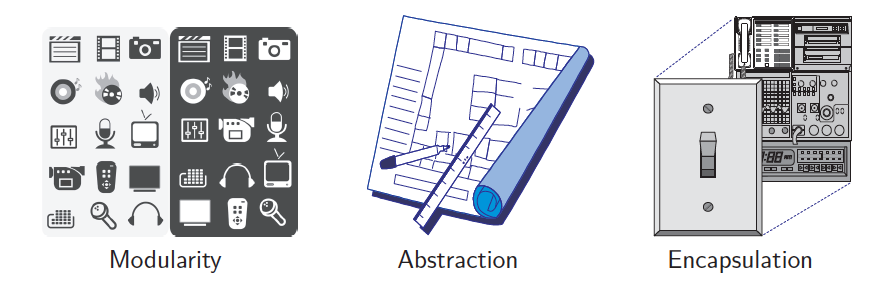
\includegraphics[width=10cm]{pic32.png}
\end{center}
\end{frame}

\begin{frame}[fragile]
  \frametitle{Principi objektno-orijentisanog dizajna $_2$}
  \begin{itemize}
    \item klasa sadrži atribute i metode
    \item $\Rightarrow$ podaci i operacije nad podacima se nalaze na jednom mestu
    \item pristup podacima je kontrolisan; mogu se menjati samo putem postojećih operacija
  \end{itemize}
\end{frame}

\begin{frame}[fragile]
  \frametitle{Šta je \texttt{\_\_init\_\_}}
\begin{minted}{python}
class Point:
    def __init__(self, x, y):
        self.x = x
        self.y = y
\end{minted}
  \begin{itemize}
    \item \texttt{\_\_init\_\_} je metoda koja se automatski poziva kada se objekat \myblue{kreira} u memoriji
    \item \myblue{konstruktor} objekta
  \end{itemize}
\end{frame}

\begin{frame}[fragile,shrink]
  \frametitle{Primer: tačka, duž, krug}
\begin{minted}{python}
import math

class Point:
    def __init__(self, x, y):
        self.x = x
        self.y = y

    def equals(self, other):
        return self.x == other.x and self.y == other.y

    def distance(self, other):
        return math.sqrt((self.x-other.x)**2 + 
            (self.y-other.y)**2)
\end{minted}
\end{frame}

\begin{frame}[fragile]
  \frametitle{Primer: tačka, duž, krug $_2$}
\begin{minted}{python}
class Circle:
    def __init__(self, center, radius):
        self.center = center
        self.radius = radius

    def contains(self, point):
        return center.distance(point) <= radius
\end{minted}
\end{frame}

\begin{frame}[fragile]
  \frametitle{Primer: tačka, duž, krug $_3$}
\begin{minted}{python}
class LineSegment:
    def __init__(self, point1, point2):
        self.point1 = point1
        self.point2 = point2
        
    def contains(self, point):
        # proveri da li je tacka na duzi
\end{minted}
\end{frame}

\section[Nasleđivanje]{Nasleđivanje}

\begin{frame}[fragile]
  \frametitle{Nasleđivanje}
  \begin{itemize}
    \item šta je zajedničko za tačku, krug i duž?
    \item svi su geometrijski pojmovi
    \item mogu se nacrtati na ekranu
    \item algoritam za crtanje nije isti u sva tri slučaja
  \end{itemize}
\end{frame}

\begin{frame}[fragile]
  \frametitle{Nasleđivanje}
  \begin{itemize}
    \item zajedničke osobine više klasa možemo grupisati u posebnu \myblue{roditeljsku} klasu
    \item postojeće klase \myblue{nasleđuju} roditeljsku klasu
    \item nasleđuju atribute i metode
    \item i mogu da dodaju specifično ponašanje
  \end{itemize}
\end{frame}

\begin{frame}[fragile]
  \frametitle{Primer: tačka, duž, krug $_4$}
\begin{minted}{python}
class Shape:
    def __init__(self):
        # zajednicki atribut
        self.color = '000000'

    def draw(self):
        # apstraktni oblik ne ume da se nacrta
        raise NotImplementedError(
            'Naslednik mora ovo da redefinise!')
\end{minted}
\end{frame}

\begin{frame}[fragile,shrink]
  \frametitle{Primer: tačka, duž, krug $_5$}
\begin{minted}{python}
class Point(Shape):
    ...
    def draw(self):
        # crtanje tacke

class Circle(Shape):
    ...
    def draw(self):
        # crtanje kruznice

class LineSegment(Shape):
    ...
    def draw(self):
        # crtanje duzi
\end{minted}
\end{frame}

\begin{frame}[fragile,shrink]
  \frametitle{Primer: tačka, duž, krug $_6$}
\begin{minted}{python}
class Point(Shape):
    def __init__(self):
        # poziv roditeljskog konstruktora
        super(Point, self).__init__()
        
    def draw(self):
        # crtanje tacke
\end{minted}
\end{frame}

\begin{frame}[fragile]
  \frametitle{Polimorfizam}
\begin{minted}{python}
# predstavlja crtez koji se sastoji iz liste figura
class Drawing:
    def __init__(self):
        # elementi liste bice naslednici Shape-a
        self.shapes = []

    def drawEverything(self):
        # prodji kroz listu Shape-ova
        for shape in self.shapes:
            # on ce sam znati kako da se nacrta
            shape.draw()
\end{minted}
\end{frame}

\begin{frame}[fragile]
  \frametitle{Polimorfizam $_2$}
\begin{minted}{python}
drawing = Drawing()
p1 = Point(3, 4)
p2 = Point(6, 7)
p3 = Point(2, 2)
ls1 = LineSegment(p1, p2)
c1 = Circle(p2, 4)
drawing.shapes.append(p3)
drawing.shapes.append(ls1)
drawing.shapes.append(c1)

drawing.drawEverything()
\end{minted}
  \begin{itemize}
    \item bez polimorfizma petlja za iscrtavanje figura bi morala da sadrži ogroman if/elif/elif/...
  \end{itemize}
\end{frame}

\begin{frame}[fragile]
  \frametitle{Strukturno vs. objektno-orijetisano programiranje}
  \begin{itemize}
    \item osnovni koncepti \textbf{strukturnog programiranja}:
    \begin{itemize}
      \item sekvenca (blok naredbi)
      \item selekcija (grananje)
      \item iteracija (petlje)
    \end{itemize}
    \item dodajmo tu još i
    \begin{itemize}
      \item modularizaciju (dekompoziciju na potprograme) \\ \ \\
    \end{itemize}
    \item \textbf{objektno-orijentisano programiranje} se oslanja na sve to i dodaje
    \begin{itemize}
      \item klase i objekte
      \item nasleđivanje
      \item enkapsulaciju
      \item apstrakciju
    \end{itemize}
  \end{itemize}
\end{frame}

\section[Primer]{Primer: studentska služba}

\begin{frame}[fragile]
  \frametitle{Primer: studentska služba}
  \begin{itemize}
    \item implementiramo referentni projekat pomoću OOP
  \end{itemize}
\begin{minted}{python}
class Student:
    def __init__(self):
        self.indeks = ''
        self.ime = ''
        self.prezime = ''
        self.roditelj = ''
        self.jmbg = ''
        self.adresa = ''
        self.telefon = ''
        self.email = ''
        self.godina = 0

    def upisi_narednu_godinu(self):
        self.godina += 1

\end{minted}
\end{frame}

\begin{frame}[fragile,shrink=10]
  \frametitle{Primer: studentska služba $_2$}
\begin{minted}{python}
class Student:
    ...
    def to_string(self):
        return "|".join(s.indeks, s.ime, s.prezime, 
            s.roditelj, s.jmbg, s.adresa, s.telefon, 
            s.email, s.godina')
    
    def from_string(line):
        # Ovo je statička metoda: nije potreban objekat 
        # da bi se pozvala
        s = Student()
        s.indeks, s.ime, s.prezime, s.roditelj, s.jmbg, 
            s.adresa, s.telefon, s.email, s.godina = \
            line.split("|")
        return s
\end{minted}
\end{frame}

\begin{frame}[fragile]
  \frametitle{Primer: studentska služba $_3$}
\begin{minted}{python}
# učitavanje studenata iz fajla
studenti = []
for line in open('studenti.txt', 'r'):
    s = Student.from_string(line[:-1])
    studenti.append(s)
\end{minted}
  \begin{itemize}
    \item gde staviti operacije nad listom studenata?
    \item $\Rightarrow$ klasa \texttt{StudentInformationService}
  \end{itemize}
\end{frame}

\begin{frame}[fragile]
  \frametitle{Primer: studentska služba $_4$}
\begin{minted}{python}
class StudentInformationService:
    def __init__(self):
        self.studenti = []

    def load(filename):
        studenti = []
        with open(filename, 'r') as student_file:
            for line in student_file.readlines():
                s = Student.from_string(line[:-1])
                self.studenti.append(s)

    def upis_naredne_godine():
        for s in self.studenti:
            if s.ima_uslov():
                s.upisi_narednu_godinu()
\end{minted}
\end{frame}

\end{document}